\documentclass[a4paper,11pt]{article}
\input{/home/tof/Documents/Cozy/latex-include/preambule_lua.tex}
\newcommand{\showprof}{show them}  % comment this line if you don't want to see todo environment
\fancyhead[L]{Ordonnancement - implémentation}
\newdate{madate}{10}{09}{2020}
\fancyhead[R]{Terminale - NSI} %\today
\fancyfoot[L]{~\\Christophe Viroulaud}
\fancyfoot[C]{\textbf{Page \thepage}}
\fancyfoot[R]{\includegraphics[width=2cm,align=t]{/home/tof/Documents/Cozy/latex-include/cc.png}}
\usepackage{tikz}

\begin{document}
\begin{Form}
\paragraph{Objectif:}Choisir une structure de données adaptée à la situation à modéliser.
\section{Problématique}
Le processeur peut adopter plusieurs stratégies pour exécuter l'enchaînement des processus. Selon l'algorithme utilisé (\emph{First Come First Served, Shortest Job First...)} la structure adoptée pour stocker la liste des tâches a une importance fondamentale.
\begin{center}
\shadowbox{\parbox{10cm}{\centering Quelles structures de données adopter pour implémenter les algorithmes d'ordonnancement?}}
\end{center}
\section{Des structures héritées de la liste chaînée}
\subsection{Pile}
\subsubsection{Présentation}
Les piles (\emph{stack} en anglais) sont fondées sur le principe du \emph{dernier arrivé premier sorti} (\emph{Last In First Out)}. L'image classique est la pile d'assiette.
\begin{figure}[!h]
\centering
\begin{tikzpicture}[scale=0.5]
\draw (0,0) grid (1,3);
\draw (-2,4) grid (-1,5);

\draw[->,>=latex] (-1,4.5) to[out=0,in=90] (0.5,3);

\draw (5,0) grid (6,3);
\draw (7,4) grid (8,5);

\draw[->,>=latex] (5.5,3) to[out=90,in=180] (7,4.5);
\end{tikzpicture}
\captionof{figure}{Empiler - dépiler}
\end{figure}
\subsubsection{Interface}
Les éléments sont \emph{empilés} ou \emph{dépilés} en respectant la règle du \emph{LIFO}. La pile doit alors proposer ces fonctionnalités. Une interface classique de pile  d'éléments de type noté \emph{T} est la suivante:
\begin{itemize}
\item \textbf{creer\_pile()$\;\rightarrow\;$Pile():} crée une pile vide
\item \textbf{est\_vide()$\;\rightarrow\;$bool:} renvoie \emph{True} si la pile est vide, \emph{False} sinon.
\item \textbf{empiler(e: T)$\;\rightarrow\;$None:} ajoute un élément \emph{e} au sommet de la pile.
\item \textbf{depiler()$\;\rightarrow\;$T:} retire et renvoie l'élément du sommet de la pile.
\end{itemize}
\subsubsection{Implémentation}
Les principes utilisés pour créer une liste chaînée sont repris ici.
\begin{activite}
\begin{enumerate}
\item Créer la classe \textbf{Nœud} similaire à la classe \emph{Maillon} déjà utilisée pour créer une liste chaînée. Elle possédera les attributs \emph{donnees} et \emph{successeur}.
\item Créer une classe \textbf{Pile} et sa méthode \textbf{\_\_init\_\_(self)}. Elle possédera un attribut \emph{dernier} initialisé à \emph{None}.
\item Créer les méthodes proposées dans l'interface.
\end{enumerate}
\end{activite}
\begin{commentprof}
\begin{itemize}
\item \textbf{creer\_pile} = \_\_init\_\_
\item \textbf{depiler} = doit gérer le cas où pile est vide (avec un raise par exemple
\end{itemize}
\end{commentprof}
\subsection{File}
\subsubsection{Présentation}
Les files (\emph{queue} en anglais) sont fondées sur le principe du \emph{premier arrivé premier sorti} (\emph{First In First Out}). L'image classique est la file d'attente.
\begin{figure}[!h]
\centering
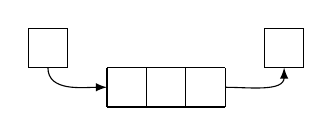
\begin{tikzpicture}[scale=0.5]
\draw (0,0) grid (3,1);
\draw (-2,1) grid (-1,2);
\draw (4,1) grid (5,2);

\draw[->,>=latex] (-1.5,1) to[out=270,in=180] (0,0.5);
\draw[->,>=latex] (3,0.5) to[out=0,in=270] (4.5,1);
\end{tikzpicture}
\captionof{figure}{Enfiler - défiler}
\end{figure}
\subsubsection{Interface}
Les éléments sont \emph{enfilés} ou \emph{défilés} en respectant la règle du \emph{FIFO}. La file doit alors proposer ces fonctionnalités. Une interface classique de file  d'éléments de type noté \emph{T} est la suivante:
\begin{itemize}
\item \textbf{creer\_file()$\;\rightarrow\;$File():} crée une file vide.
\item \textbf{est\_vide()$\;\rightarrow\;$bool:} renvoie \emph{True} si la file est vide, \emph{False} sinon.
\item \textbf{enfiler(e: T)$\;\rightarrow\;$None:} ajoute un élément \emph{e} à l'arrière de la file.
\item \textbf{defiler()$\;\rightarrow\;$T:} retire et renvoie l'élément de l'avant de la file.
\end{itemize}
\subsubsection{Implémentation}
Ici encore une classe \emph{Nœud} sera utilisée pour créer les éléments
\begin{activite}
\begin{enumerate}
\item Récupérer la classe \textbf{Nœud}. 
\item Créer une classe \textbf{File} et sa méthode \textbf{\_\_init\_\_(self)}. Elle possédera deux attributs: \emph{premier} et \emph{dernier}.
\item Créer les méthodes proposées dans l'interface.
\end{enumerate}
\end{activite}
\section{Ordonnancement}
Reprenons certains algorithmes d'ordonnancement.
\begin{activite}
\begin{enumerate}
\item Rappeler le principe du \emph{First Come First Served}. Quelle structure semble adaptée à cet algorithme?
\item Même question pour le \emph{Round Robin}.
\end{enumerate}
\end{activite}
\begin{commentprof}
Shortest First Job: il y a un calcul du temps d'exécution à chaque requête du CPU; si égalité on a une FIFO.
\end{commentprof}
\end{Form}
\end{document}